\Chapter{A dokumentum strukturális elemzése}

Elkészítettem egy olyan programot, amely beolvassa a megadott PDF dokumentumot, majd az oldalait PNG kiterjesztésű képpé konvertálja és lementi a megadott mappába.
Ez a programban a következőképpen hajtható végre.

\begin{python}
images = convert_from_path('pdf_files/testpdf.pdf')
numberOfPages = len(images)
for i in range(numberOfPages):
    images[i].save('images/test' + format(i) + '.png', 'PNG')
\end{python}

Amint megvannak az oldalak, beolvassa őket, majd fekete-fehér képpé alakítja mindegyiket. Kezdeti lépésnek a margók levágását majd a paragrafusokra bontást, később pedig a sorokra, szavakra, majd betűkre bontás volt a cél. Jelenleg a paragrafusokra bontás már stabilan működik.

Ahhoz, hogy meg tudjam állapítani, hogy hol kezdődik a szöveg, és hol található összefüggő fehér rész (margó, sorköz stb.), intenzitást kellett számolnom a kép minden sorára és oszlopára (255: fehér, 0: fekete). Ehhez összeadtam a pixelek értékeit, majd elosztottam azok számával. Ezzel eredményül kaptam egy $x$ és egy $y$ tengely menti tömböt, amelyek az oszlopok és a sorok menti intenzitás átlagokat tartalmazzák.

\begin{python}
intensity_y = img_gray.sum(axis=1) / width
intensity_x = img_gray.sum(axis=0) / height
\end{python}

Ezt a két intenzitást \aref{fig:mf_2}. ábrával szemlélteti a program, amit le is ment a megadott mappába.

\begin{figure}[h]
\centering
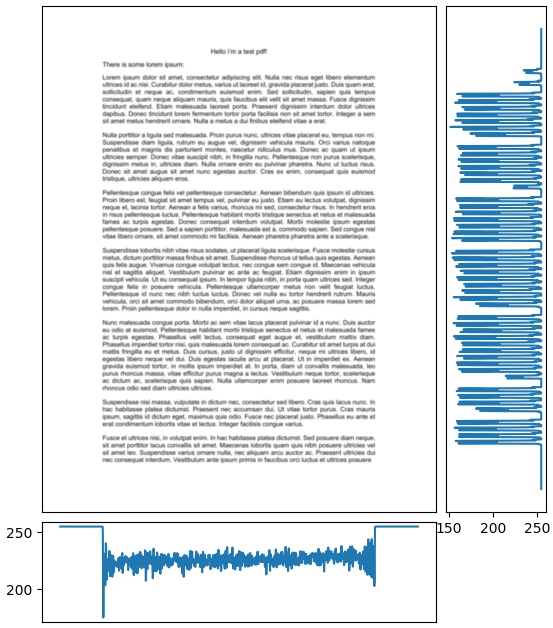
\includegraphics[scale=1]{images/mf_2.png}
\caption{A szegélyekre aggregált intenzitás értékek}
\label{fig:mf_2}
\end{figure}

Ezt a két tengely menti intenzitás tömböt felhasználva már meg lehet állapítani, melyik pixelnél ér véget a margó és hol kezdődik a szöveg. Egy egyszerű ciklussal megvizsgálom a tömb elejétől indulva hogy meddig egyenlőek az intenzitások a 255 értékkel, majd lementem azt az indexet ahol megáll a programom. Ezt megismétlem a tömbön visszafelé haladva is, így lesz meg az alsó-felső, jobb-bal margó végpontja. Ezeket felhasználva a programom eltávolítja a margókat, majd lementi a képet a megadott mappába.

\begin{python}
im1 = test.crop((left_margin,
                 height - top_margin,
                 right_margin,
                 height - bottom_margin))
im1.save('img_crop_margin/testcrop.png', 'PNG')
\end{python}

A paragrafusokra bontás is hasonlóan működik. Elindulok a tömbömön, majd egy változóban számolom hogy hány 255 értékkel egyenlő intenzitást talál egymás után a program. Ha ez több mint 10 (tapasztalati érték) akkor hozzáadja egy tömbhöz a fehér szakasz kezdőpontját (\texttt{index - 10}), majd az ehhez tartozó végpontot (amint 255 értéktől eltérő intenzitást talál, lementi az előző indexet). Így lesz egy tömböm, ami egymás után tartalmazza egy-egy bekezdésnek a kezdő majd végpontját ($y$ tengely mentén). Ezután egy ciklussal szépen kivágom a paragrafusokat.
